\documentclass{standalone}
\usepackage{fontspec}
\setsansfont{DejaVuSans.ttf}[Path=./,Kerning=Off,Ligatures={TeXOff,NoCommon}]
\usepackage{tikz}
\begin{document}
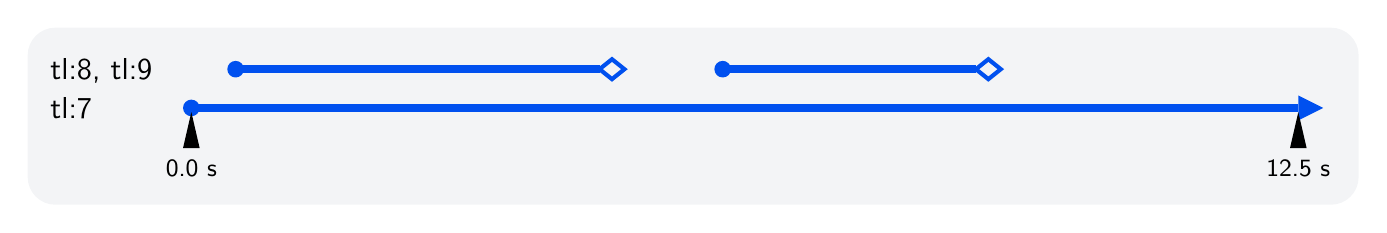
\begin{tikzpicture}[x=1pt,y=1pt,miter limit=4,font=\sffamily]
\definecolor{ts000000}{HTML}{000000}
\definecolor{ts0050EF}{HTML}{0050EF}
\definecolor{tsF3F4F6}{HTML}{F3F4F6}
\begin{scope}[shift={(16,16)}]
\path[rounded corners=10pt,fill=tsF3F4F6] (0,0) rectangle (480.9351,63.9766);
\path[draw=ts0050EF,line width=3pt] (59.1406,34.9766) -- (459.1406,34.9766);
\path[fill=ts0050EF] (59.1406,34.9766) circle[radius=3];
\path[fill=ts0050EF] (468.1406,34.9766) -- (459.1406,39.4766) -- (459.1406,30.4766) -- cycle;
\path[draw=ts0050EF,line width=3pt] (75.1406,48.9766) -- (206.6406,48.9766);
\path[fill=ts0050EF] (75.1406,48.9766) circle[radius=3];
\path[draw=ts0050EF,line width=1.5pt] (206.6406,48.9766) -- (211.1406,52.5766) -- (215.6406,48.9766) -- (211.1406,45.3766) -- cycle;
\path[draw=ts0050EF,line width=3pt] (251.1406,48.9766) -- (342.6406,48.9766);
\path[fill=ts0050EF] (251.1406,48.9766) circle[radius=3];
\path[draw=ts0050EF,line width=1.5pt] (342.6406,48.9766) -- (347.1406,52.5766) -- (351.6406,48.9766) -- (347.1406,45.3766) -- cycle;
\path[fill=ts000000] (59.1406,33.4766) -- (56.1406,20.4766) -- (62.1406,20.4766) -- cycle;
\path[fill=ts000000] (459.1406,33.4766) -- (456.1406,20.4766) -- (462.1406,20.4766) -- cycle;
\node[anchor=base west,inner sep=0,font=\sffamily\fontsize{11}{12.8047}\selectfont,text=ts000000] at (8,45.1685) {tl:8, tl:9};
\node[anchor=base west,inner sep=0,font=\sffamily\fontsize{11}{12.8047}\selectfont,text=ts000000] at (8,31.1685) {tl:7};
\node[anchor=base,inner sep=0,font=\sffamily\fontsize{9}{10.4766}\selectfont,text=ts000000] at (59.1406,10.1226) {0.0 s};
\node[anchor=base,inner sep=0,font=\sffamily\fontsize{9}{10.4766}\selectfont,text=ts000000] at (459.1406,10.1226) {12.5 s};
\end{scope}
\end{tikzpicture}
\end{document}
